% !TEX root = univariate.tex 
\begin{table}[!htbp] \centering  
\caption{}  
\label{}  
\begin{tabular}{@{\extracolsep{5pt}}lccccccc}  
\\[-1.8ex]\hline 
\hline \\[-1.8ex]  
Statistic & \multicolumn{1}{c}{Mean} & \multicolumn{1}{c}{St. Dev.} & \multicolumn{1}{c}{Min} &  \multicolumn{1}{c}{Max} \\ 
\hline \\[-1.8ex]  
hits & 86.618 & 99.984 & 9 & 800 \\ 
newVisits & 0.692 & 0.462 & 0 & 1 \\ 
pageviews & 16.313 & 14.863 & 1 & 137 \\ 
totalTransactionRevenue & 92,534.270 & 81,442.280 & 8,950 & 871,380 \\ 
transactions & 1.107 & 0.483 & 1 & 6 \\ 
timeOnSite & 888.189 & 959.672 & 0 & 7,547 \\ 
browser\_width & 1,146.060 & 653.819 & 320 & 2,560 \\ 
browser\_height & 764.110 & 156.292 & 280 & 1,356 \\ 
itemCount & 4.019 & 3.252 & 1 & 18 \\ 
\hline \\[-1.8ex]  
\end{tabular} 
\end{table}  
Dans la figure \ref{univarie_ref} nous faisons une analyse univarié de chacune des variables. 
\begin{figure}[H] 
\centering 
\subfloat[Hits: 90 \% de l’échantillon ont moins de 200 hits dans la session où ils ont effectué au  moins une transaction.]{ 
\label{hits} 
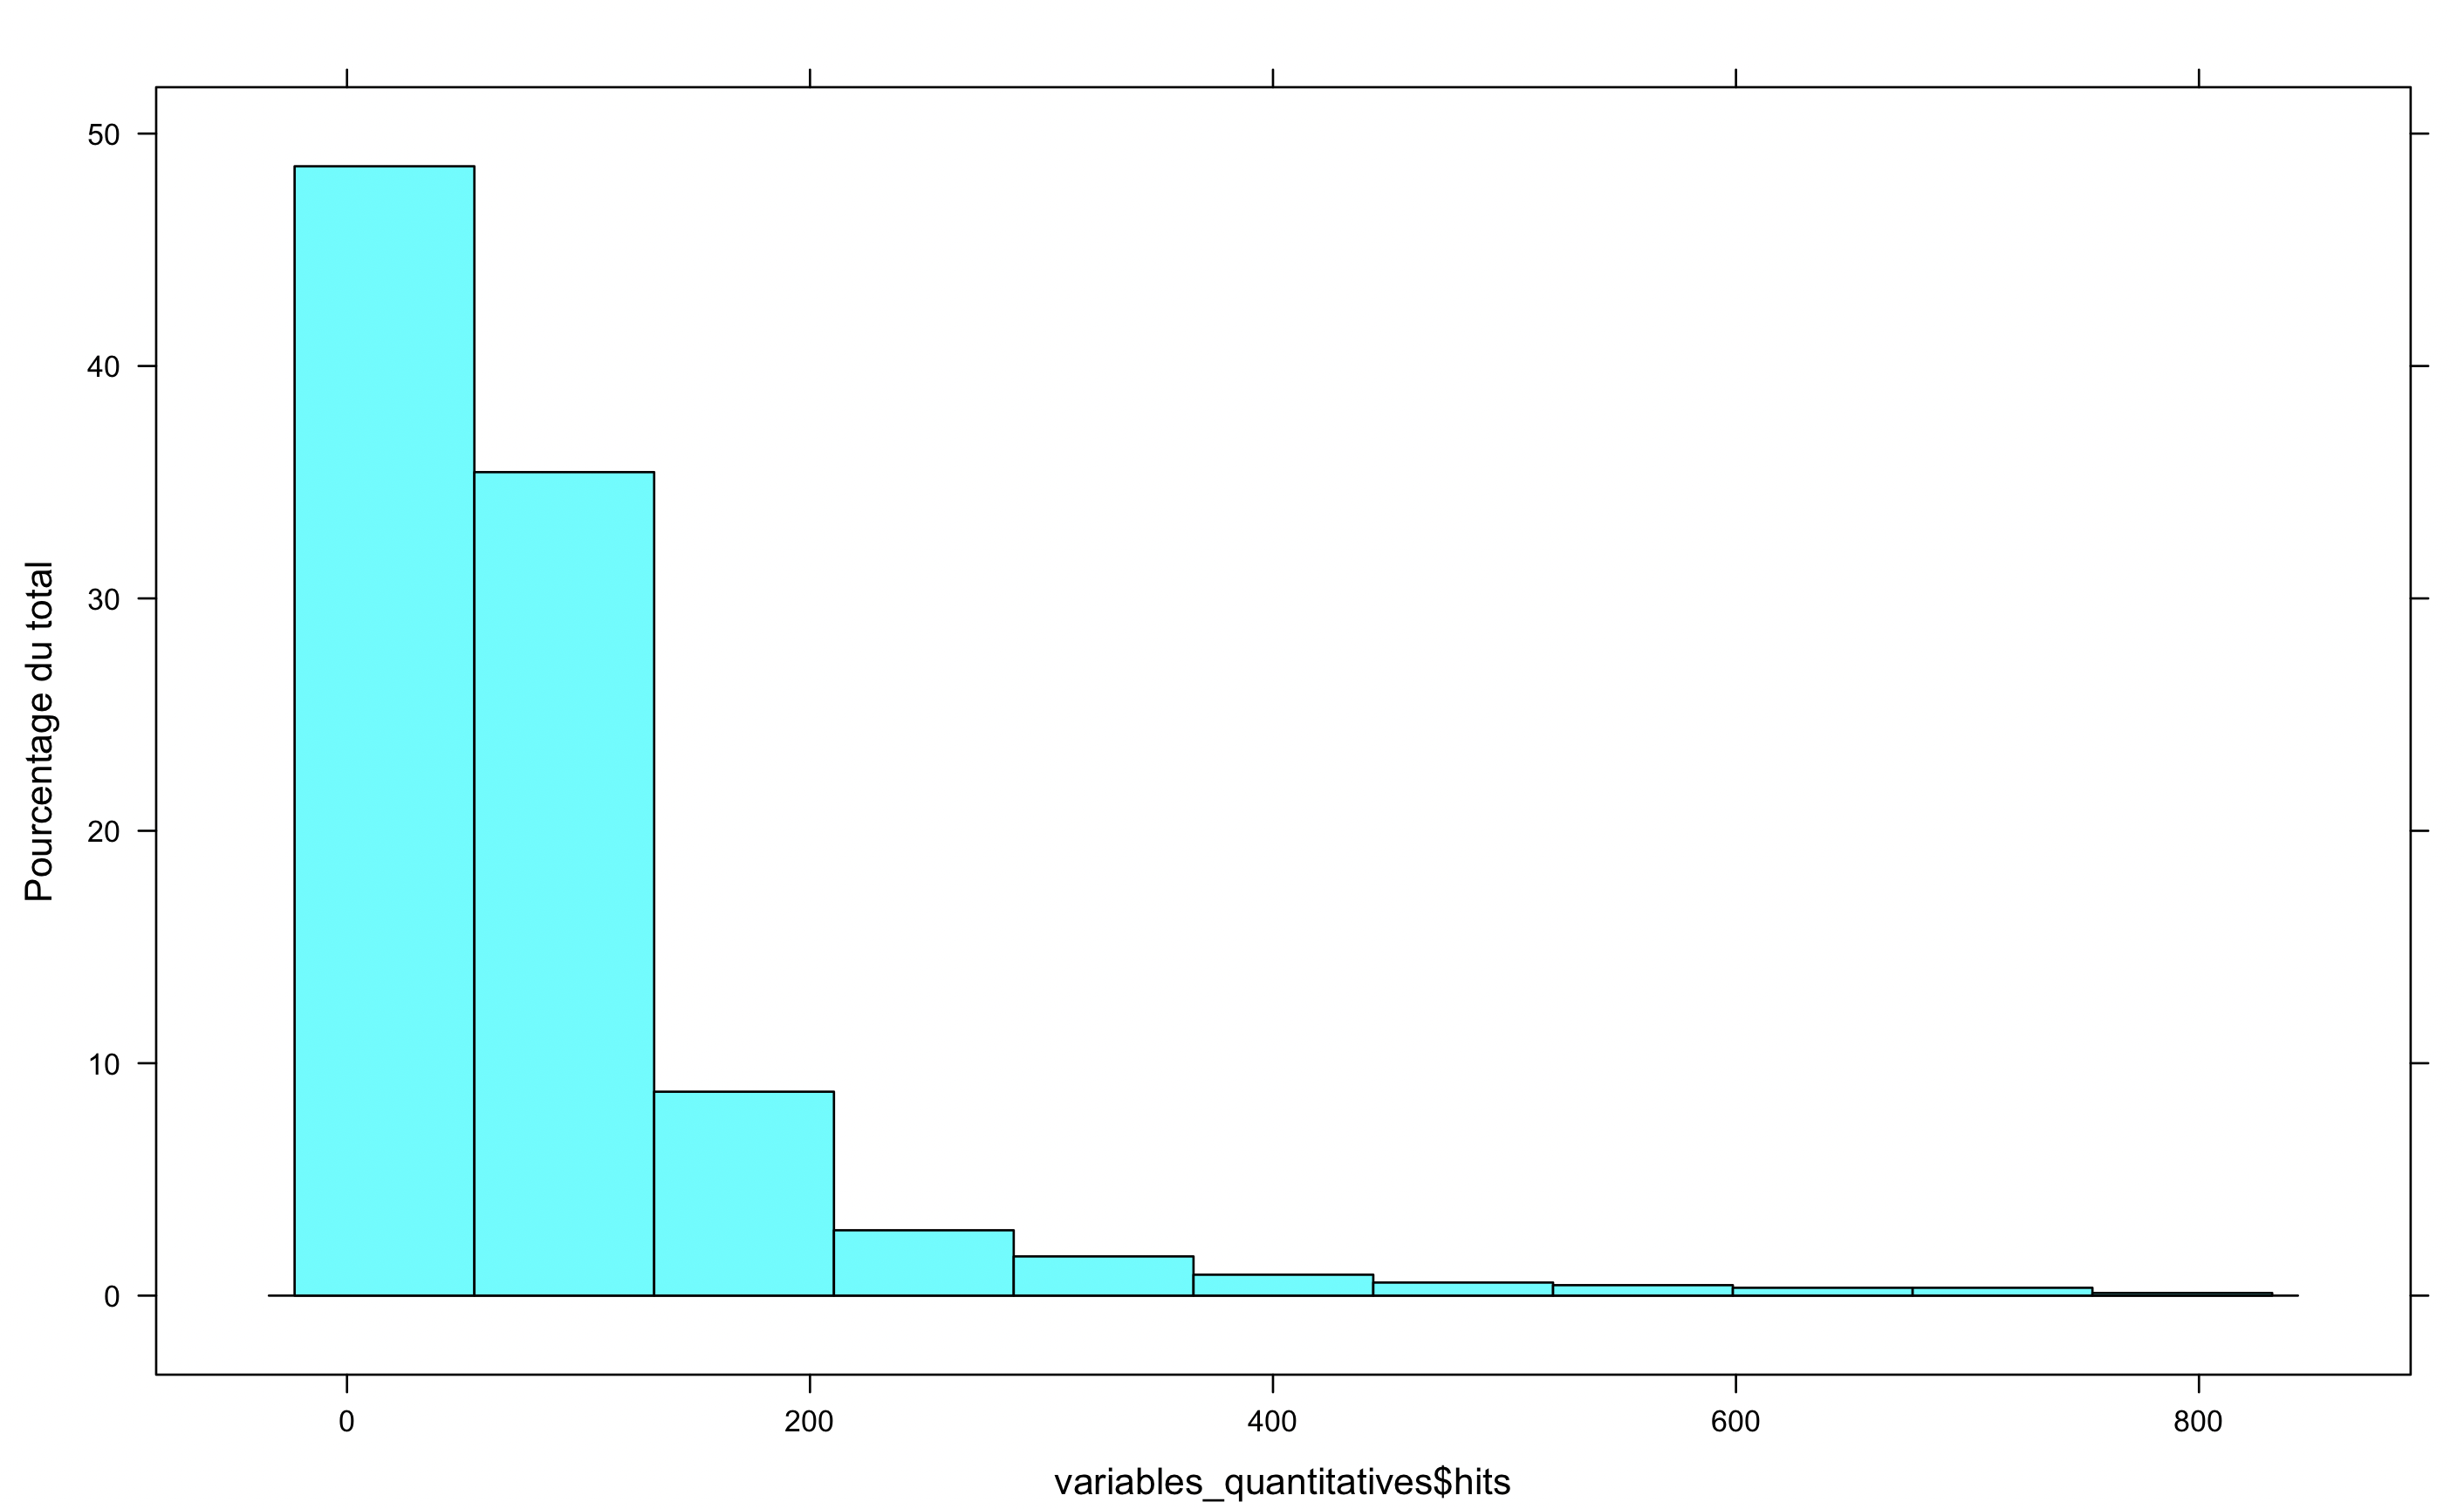
\includegraphics[width=0.45\textwidth]{scriptsR/imgs/univarie/hits_percent.png} }s 
\hfill 
\subfloat[NewVisit: 70 \% des transactions ont été réalisées par des nouveaux utilisateurs.]{ \label{new_visit} 
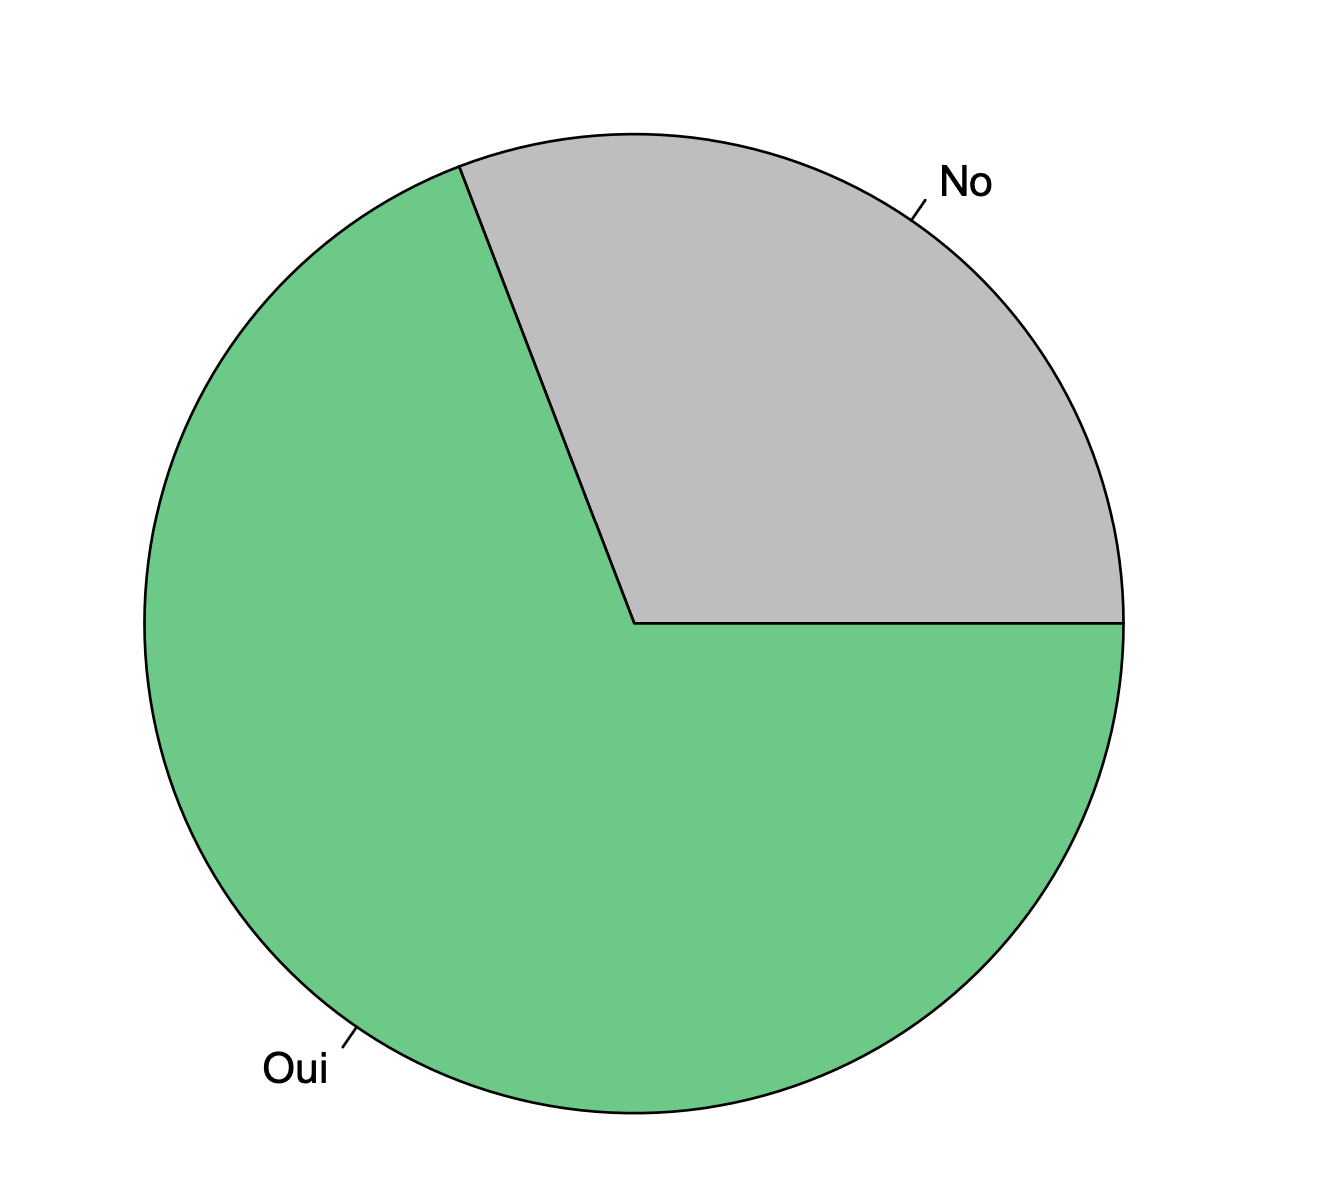
\includegraphics[width=0.45\textwidth]{scriptsR/imgs/univarie/newVisit.png} } 
\hfill 
\subfloat[PageViews: 80 \% de l’échantillon ont consultés entre 0 et 25 pages avant la transaction. ]{ \label{page_views} 
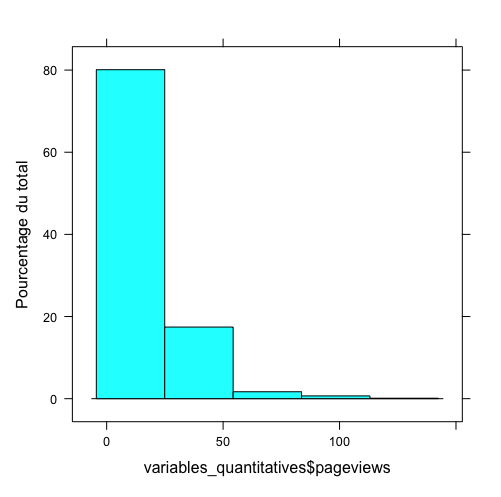
\includegraphics[width=0.45\textwidth]{scriptsR/imgs/univarie/pageviews.png} } 
\hfill 
\subfloat[TransactionsRevenue: La majorité de transactions valent entre 0\euro et 100\euro , Nous  avons aussi des transactions atypiques qui arrivent jusqu'à 800\euro ]{ 
\label{transaction_revenue} 
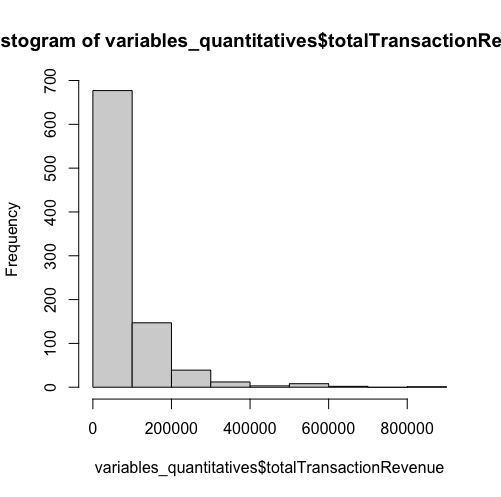
\includegraphics[width=0.45\textwidth]{scriptsR/imgs/univarie/transactionsrevenue.png} } 
\hfill 
\subfloat[Transactions : La majorité des individus font 1 transaction dans la session, ce qui  correspond à la quantité attendue. Nous laissons donc de côté cette valeur] { \label{transactions} 
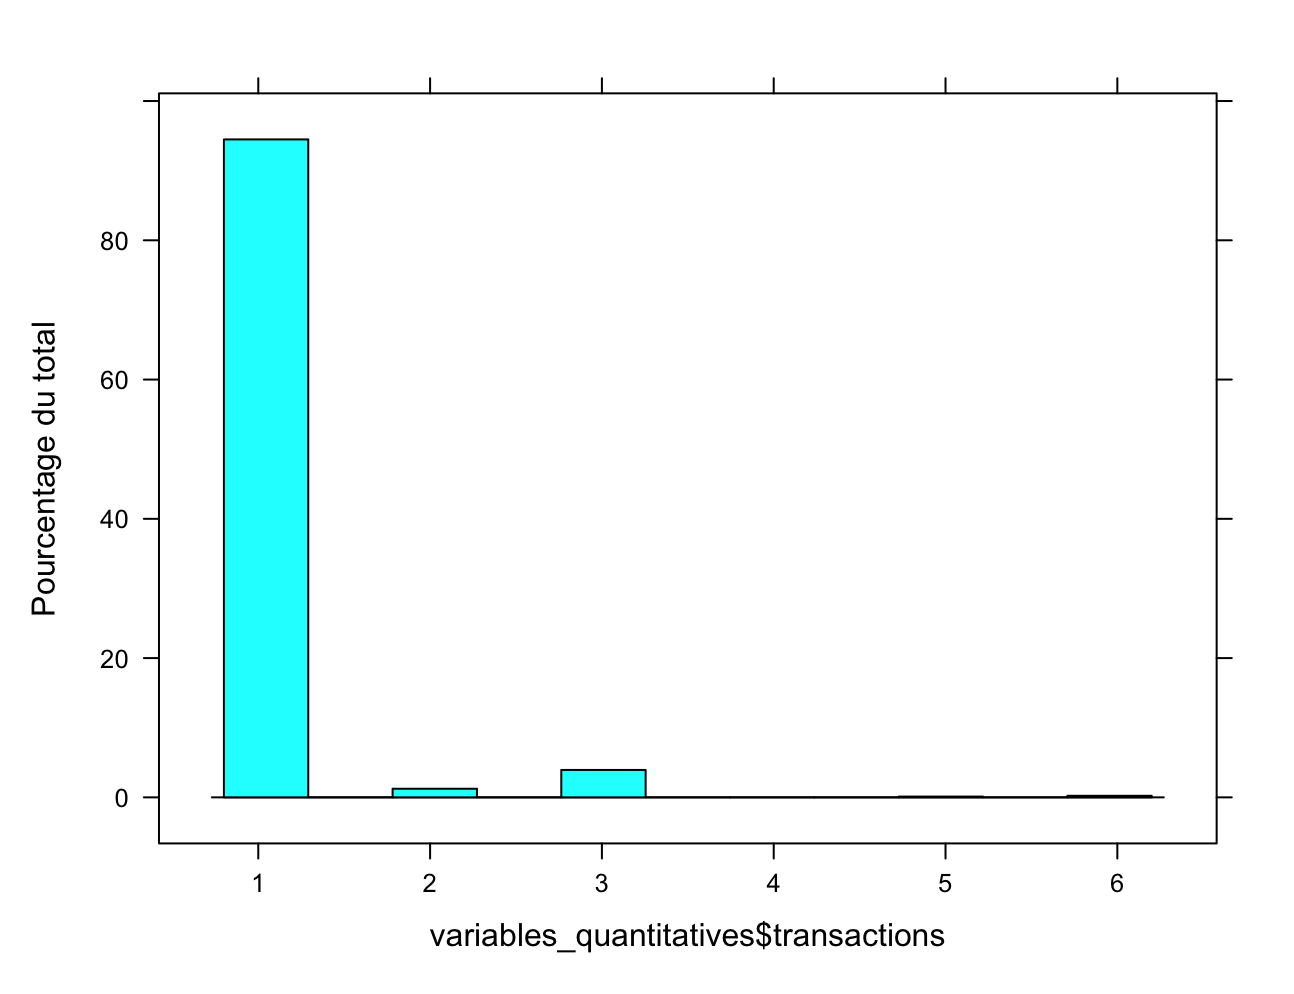
\includegraphics[width=0.45\textwidth]{scriptsR/imgs/univarie/transactionsHistogram.png} } 
\hfill 
\subfloat[ TimeOnSIte: Les individus prennent moins de 16 minutes (1000s) pour effectuer au moins  une transaction] { 
\label{timeOnSite} 
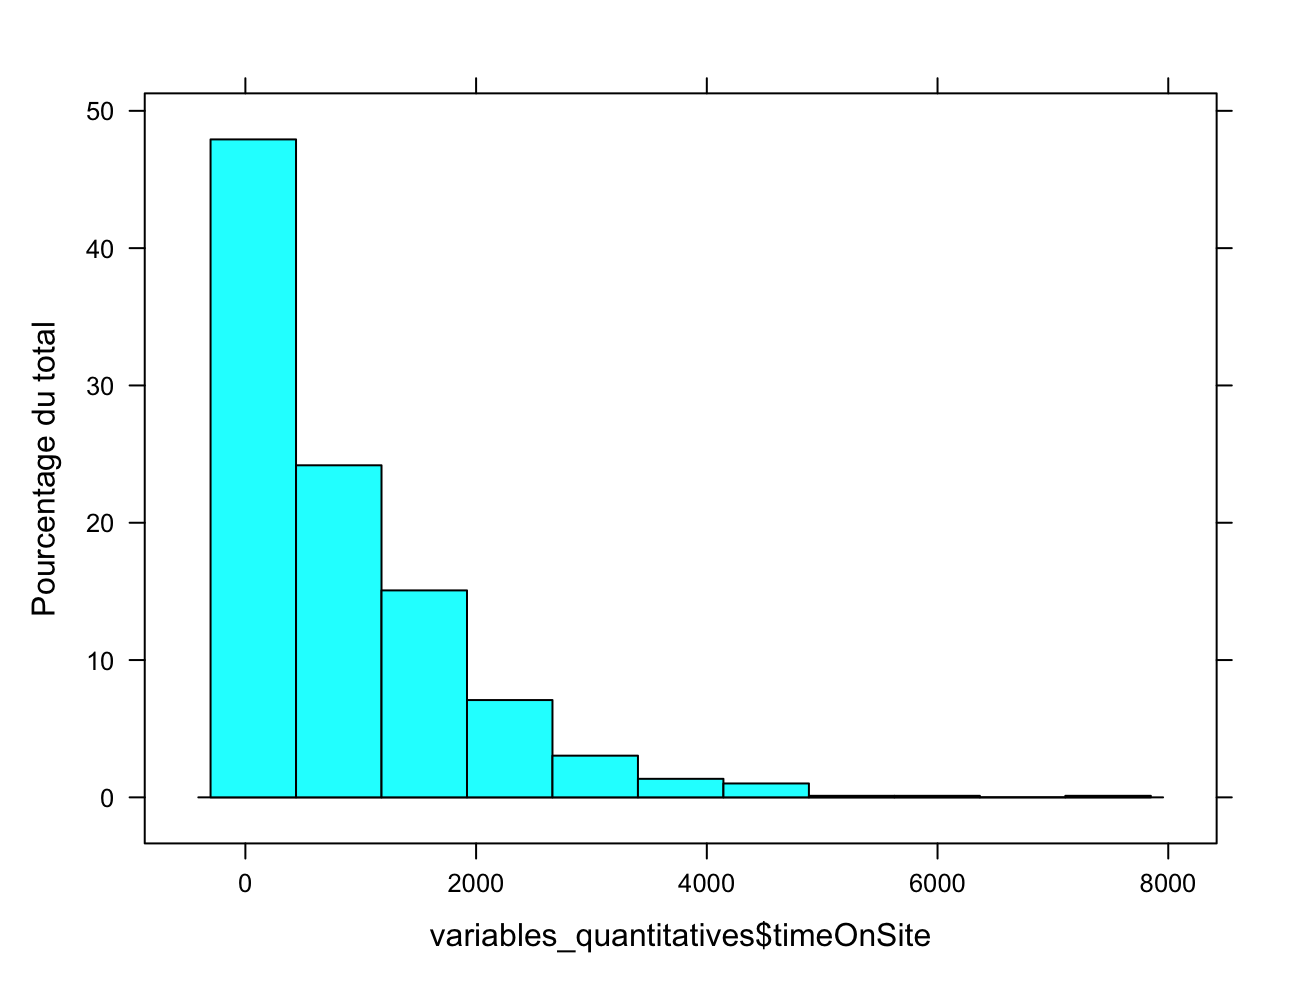
\includegraphics[width=0.45\textwidth]{scriptsR/imgs/univarie/TimeOnSIteHist.png} } 
\caption{Images Univariée 1} 
\label{univarie_ref} 
\end{figure} 




\begin{figure}[H]
\ContinuedFloat 
\centering 
\subfloat[ browserName: Chrome est le navigateur le plus utilisé de l’échantillon, suivi de safari, et  de la version mobile de chrome.] { 
\label{browserName} 
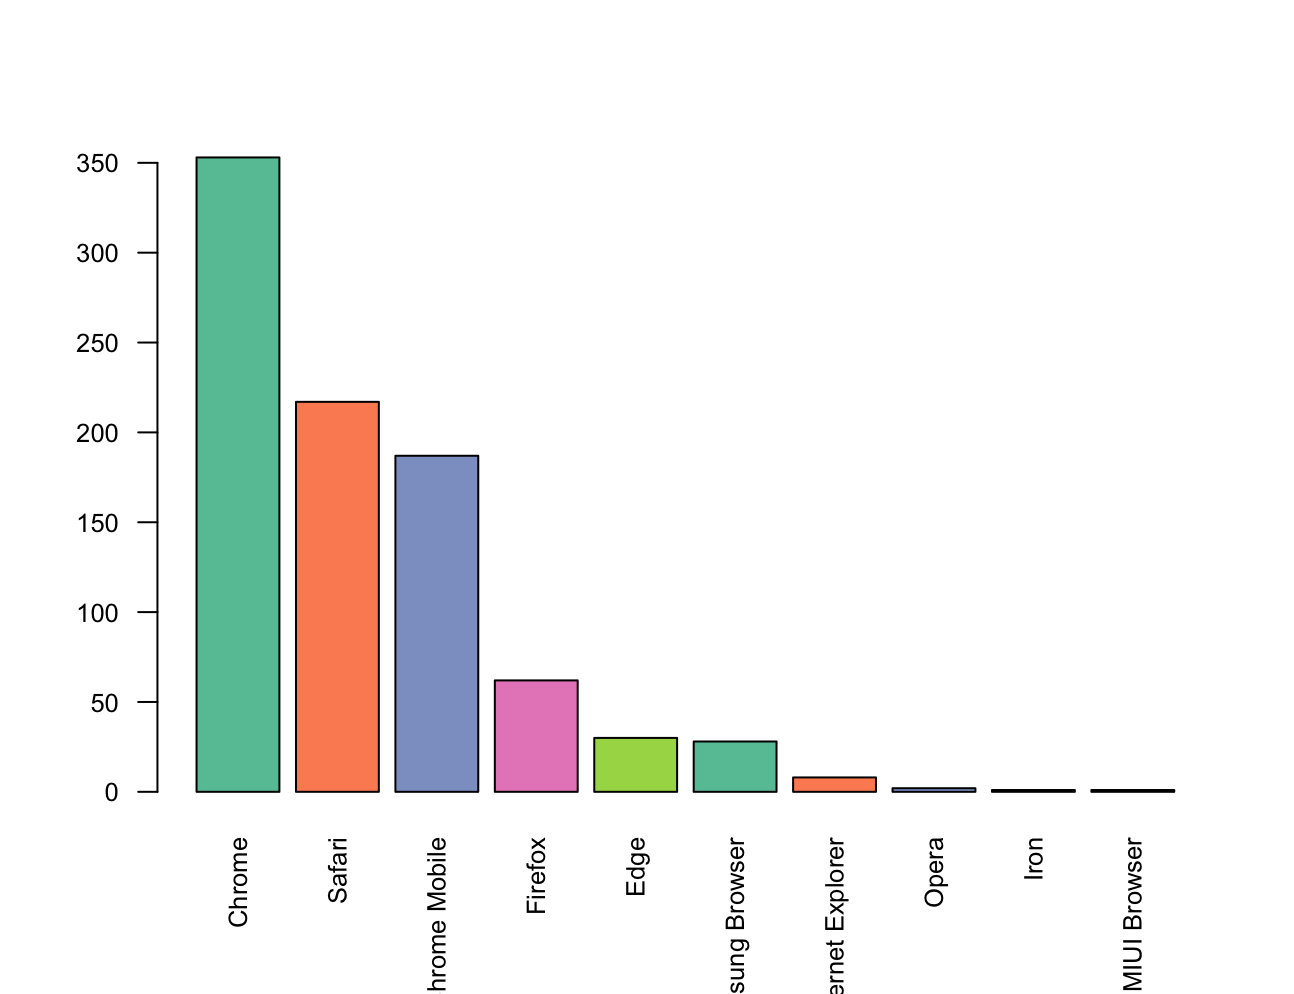
\includegraphics[width=0.45\textwidth]{scriptsR/imgs/univarie/browser_name.png} } 
\hfill 
\subfloat[ browserWidth: Il existe un pourcentage important d'individus qui ont effectué une  transaction à partir d'un écran dont la largeur est inférieure à 500, nous pouvons en déduire qu'ils  ont été réalisés depuis un appareil mobile, suivi d'une autre plage comprise entre 1800 et 1900.]{ \label{browser_widthBoxplot} 
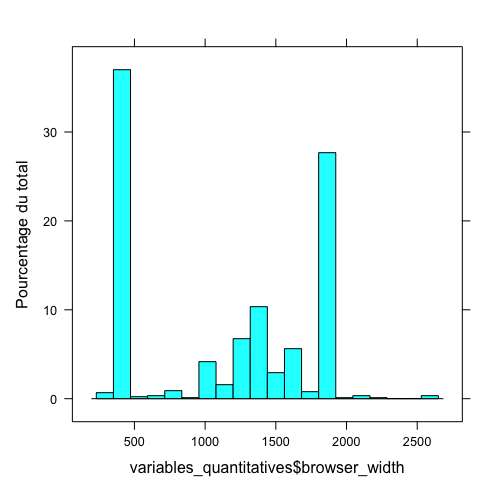
\includegraphics[width=0.45\textwidth]{scriptsR/imgs/univarie/browser_width.png} } 
\hfill 
\subfloat[ browserHeight: les données sont distribuées d'une manière plus uniforme, nous  remarquons que la plupart des largeurs d'écrans sont entre 600 pixels et 1000 pixels, nous  n'observons pas de données exceptionnelles]{ 
\label{browser_height_bloxplot} 
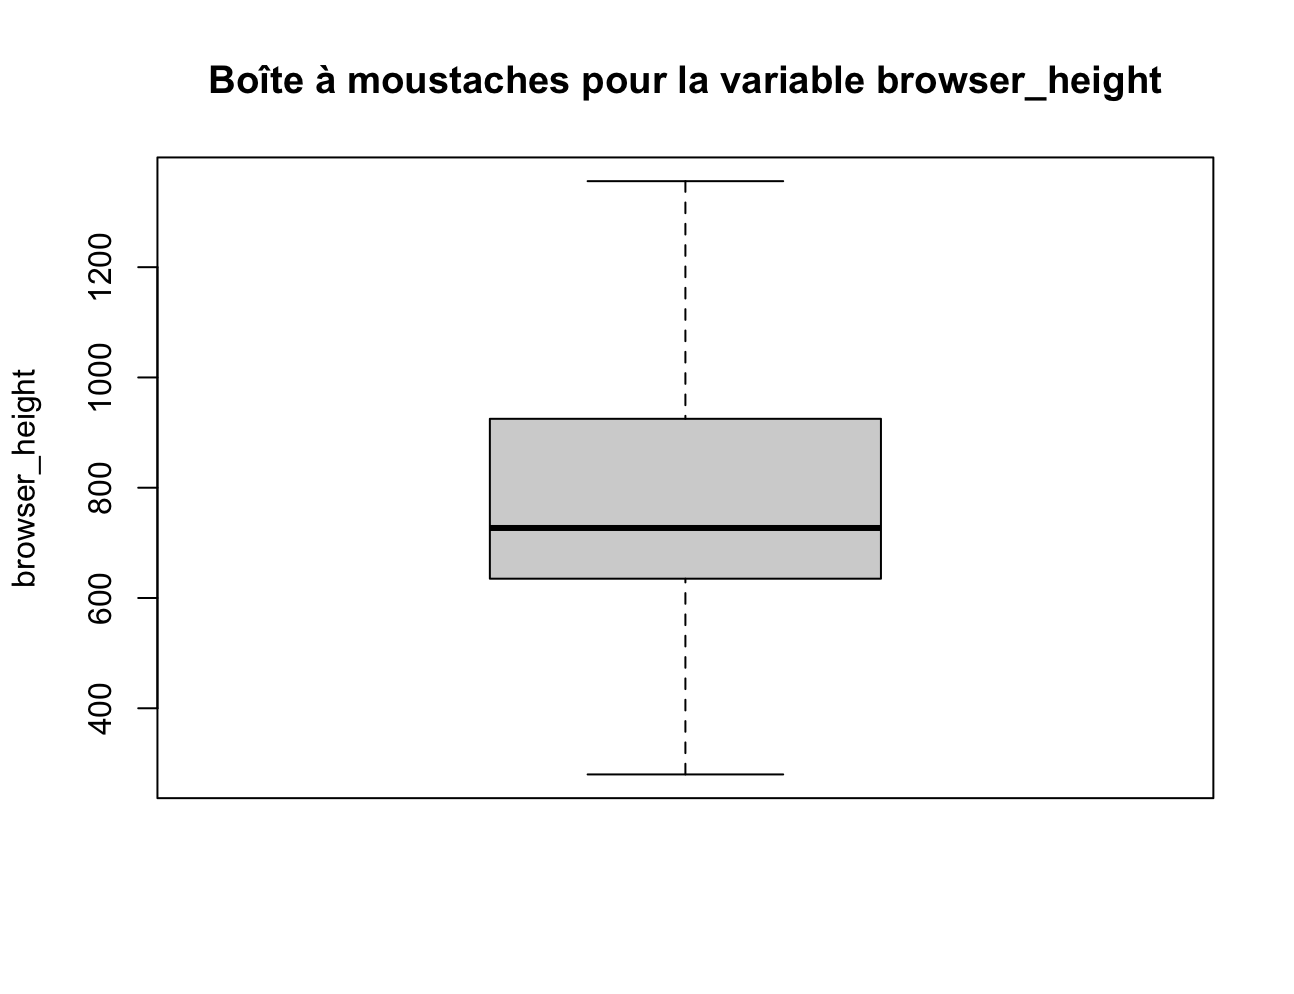
\includegraphics[width=0.45\textwidth]{scriptsR/imgs/univarie/browser_height_bloxplot.png} } 
\hfill 
\subfloat[deviceCategory: Contrairement à ce que nous avons constaté avec les autres variables, les  57 \% des transactions ont été réalisé depuis un laptop, suivi de 38\% avec un dispositif mobile.]{ \label{deviceCategory} 
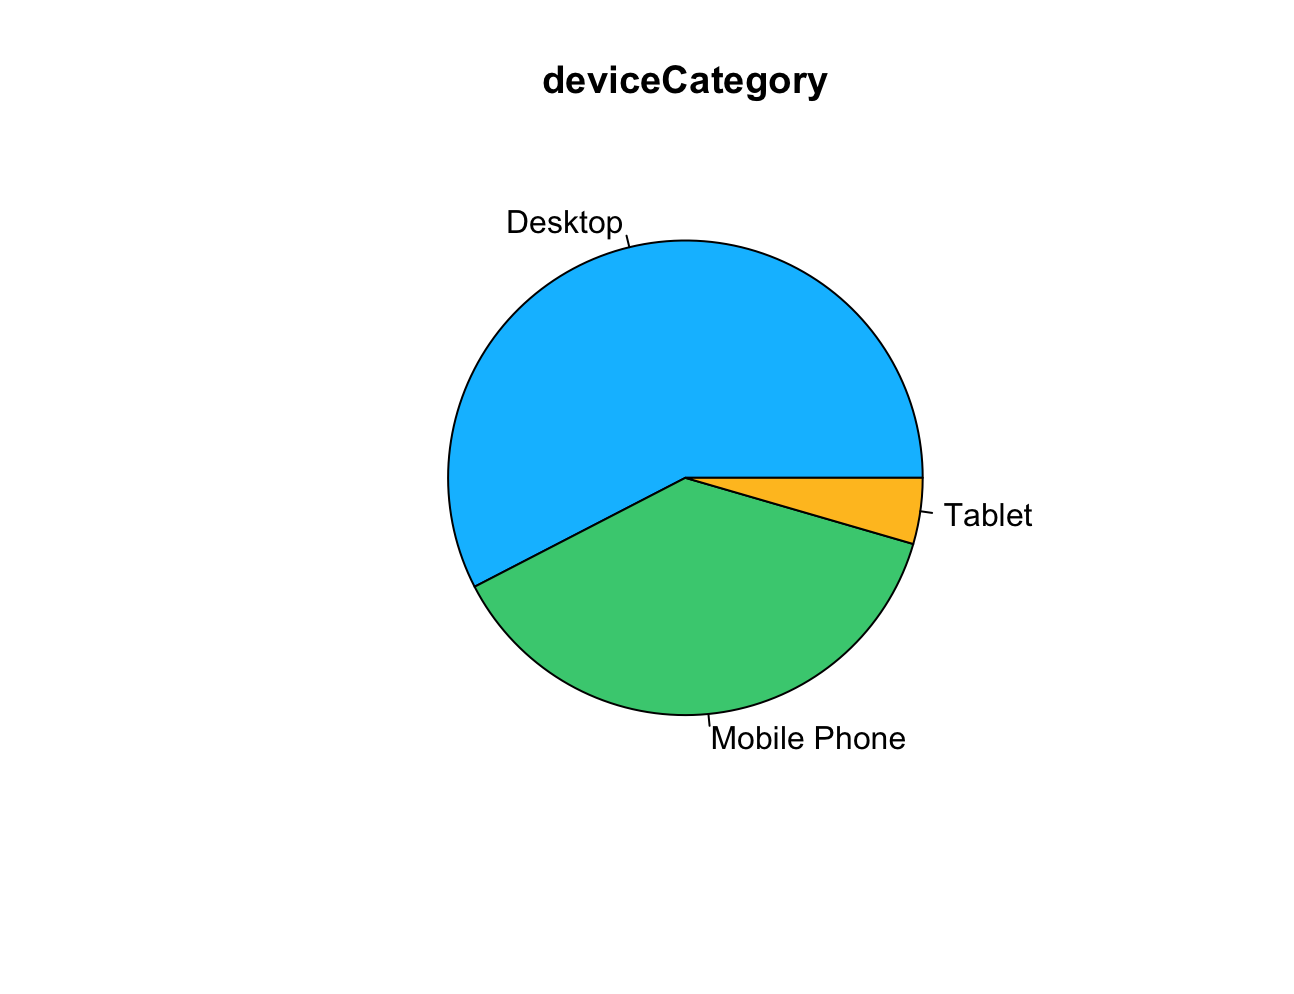
\includegraphics[width=0.45\textwidth]{scriptsR/imgs/univarie/deviceCategory.png} } 
\hfill 
\subfloat[operatingSys: Windows 10 est le système d'exploitation préféré de l’échantillon. ]{ \label{operatingSys} 
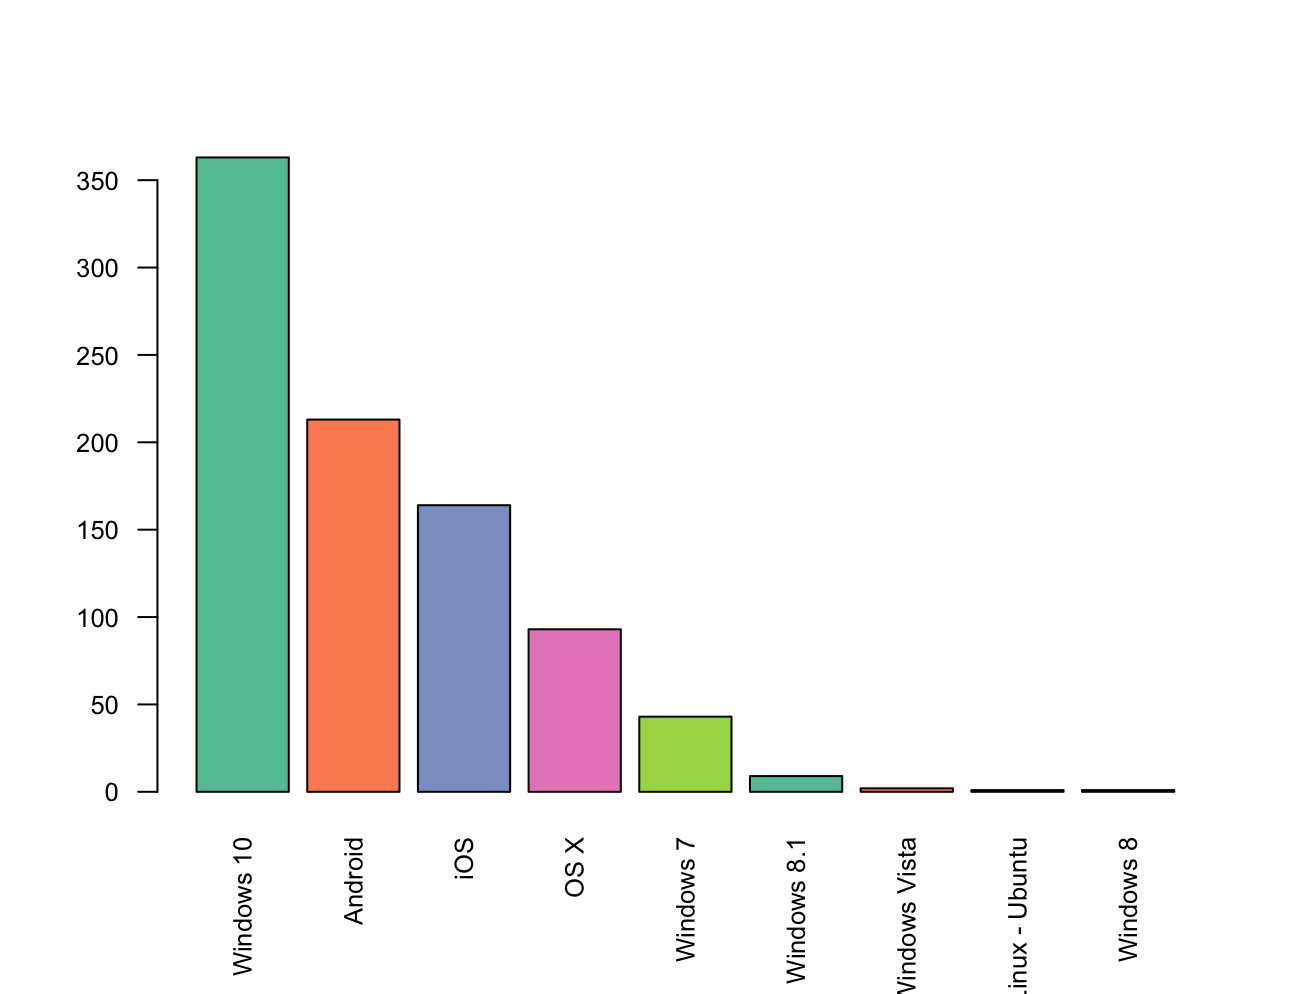
\includegraphics[width=0.45\textwidth]{scriptsR/imgs/univarie/operatingSys.png} } 
\hfill 
\subfloat[languageApply: L'anglais américain et le français de France sont les langues préférées des  utilisateurs lorsqu'ils effectuent une transaction.]{ 
\label{language} 
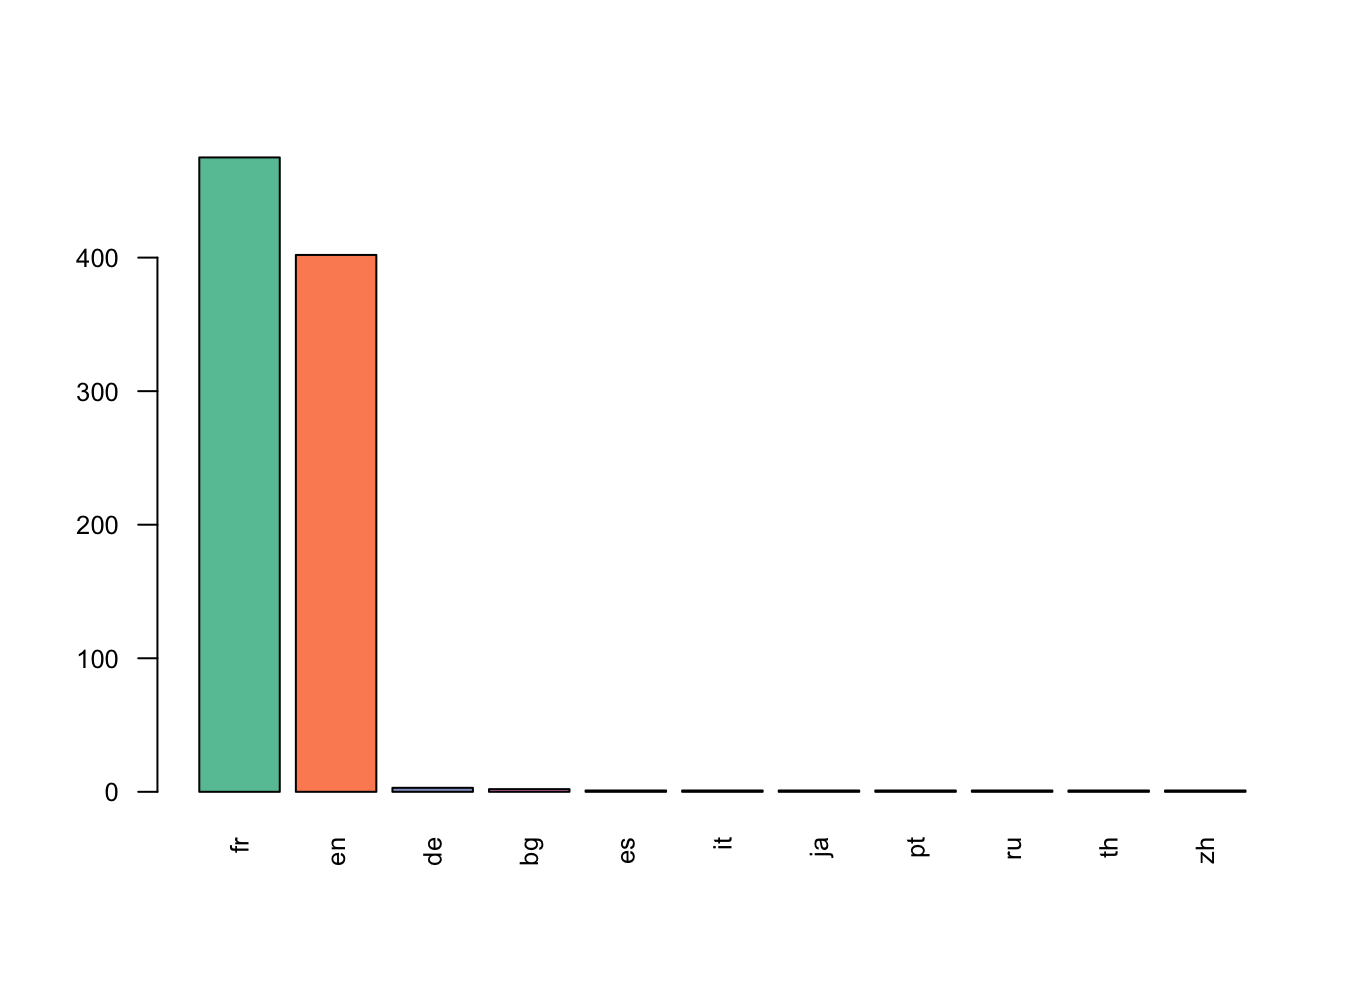
\includegraphics[width=0.45\textwidth]{scriptsR/imgs/univarie/language_apply.png} } 
\caption{Images Univariée 2 } 
\label{univarie_ref} 
\end{figure} 


\begin{figure}[H] 
\ContinuedFloat 
\centering 
\subfloat[PaymentMethod: Avec plus de 600 sessions, la carte de crédit est le mode de paiement le  plus utilisé pour les transactions, suivi de Paypal avec un peu plus de 100 session. ]{
\label{paymentMethod} 
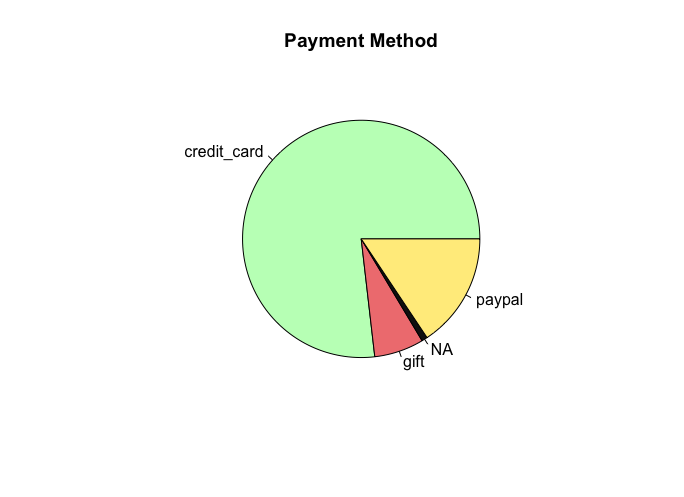
\includegraphics[width=0.45\textwidth]{scriptsR/imgs/univarie/paymentMethod.png} } 
\hfill 
\subfloat[itemCount: Dans un peu plus de la moitié des sessions, les transactions effectuées  comprenaient 1, 2 ou 3 articles, mais un nombre important des transactions contenait entre 5 et 10  articles. ]{ 
\label{itemcountHistogram} 
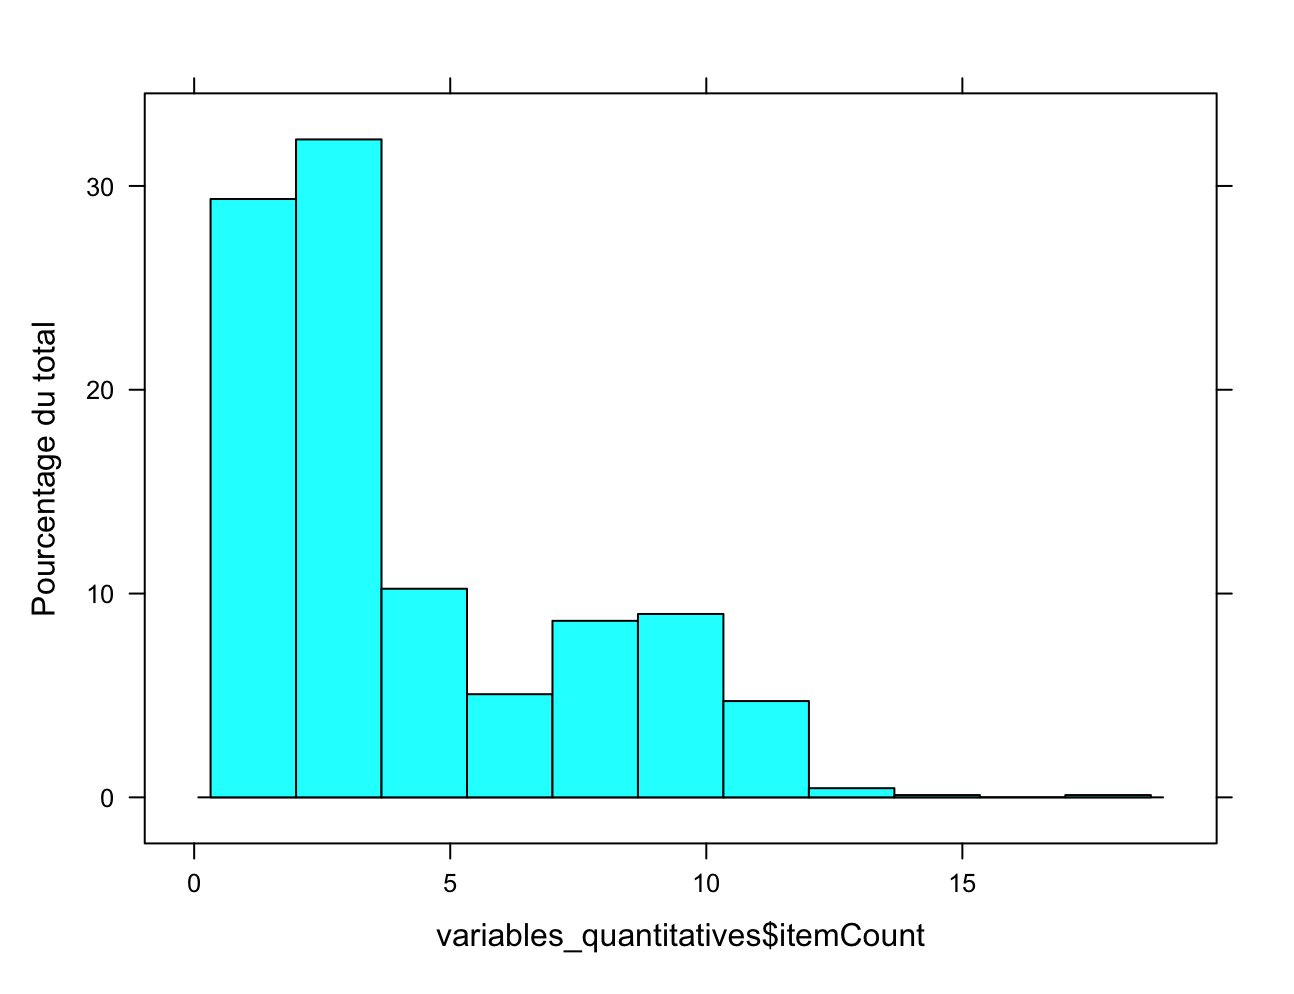
\includegraphics[width=0.45\textwidth]{scriptsR/imgs/univarie/itemcountHistogram.png} } 
\hfill 
\subfloat[Country : La France est le pays où se réalise le plus de transactions pour cet e-commerce :  501, suivi de Netherlands avec 190. Les données sont complètement cohérentes au vu de l’origine  français de cet e-commerce. ]{ 
\label{country} 
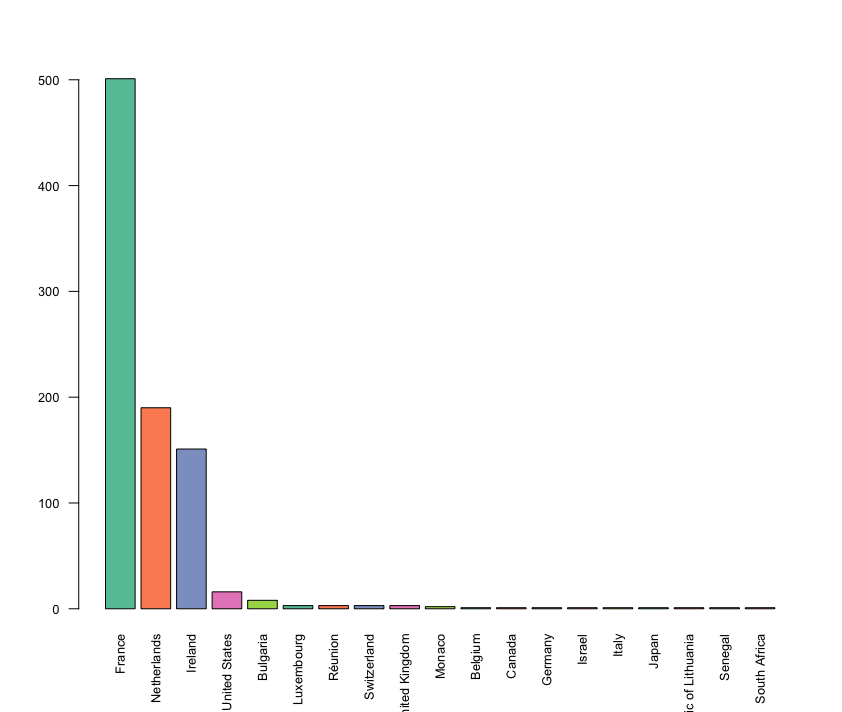
\includegraphics[width=0.45\textwidth]{scriptsR/imgs/univarie/country.png} } 
\hfill 
\subfloat[City: Nous avons 302 villes différentes dans l'échantillon et 309 transactions sans  informations sur la ville. La ville au plus grand nombre de transactions est Paris avec 90 transactions,  suivi de Dublin avec 38 transactions. ]{ 
\label{cities} 
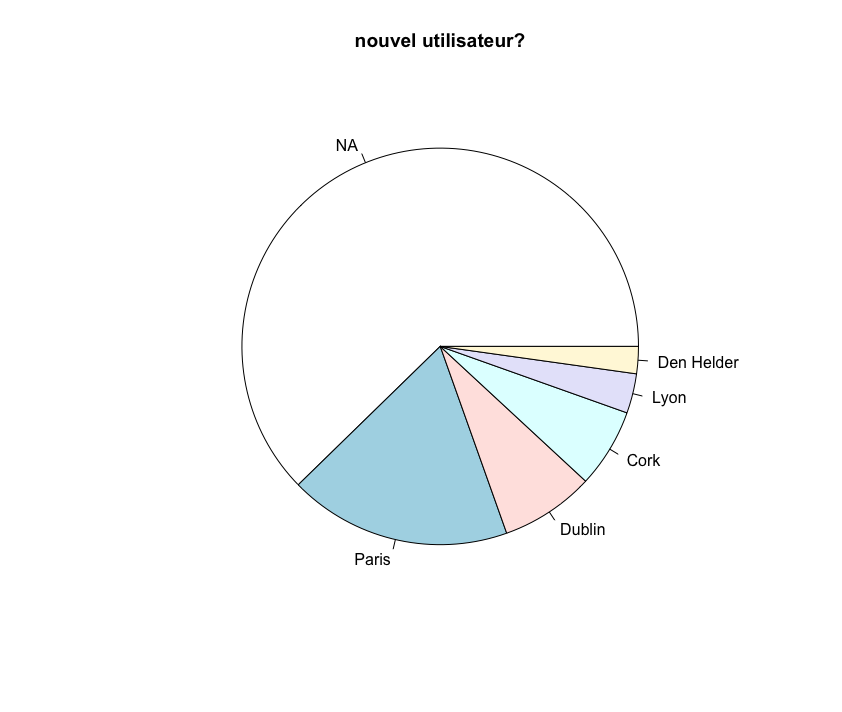
\includegraphics[width=0.45\textwidth]{scriptsR/imgs/univarie/city.png} 
} 
\caption{Images Univariée 3} 
\label{univarie_ref} 
\end{figure} 
